\subsubsection{Procesamiento y modelado de los datos}

El análisis de latencias se ha realizado mediante la 
construcción de un modelo secuencial del sistema, 
representado como un pipeline de eventos: 
\textit{Decisión $\rightarrow$ 
Arbitraje $\rightarrow$ Ejecución $\rightarrow$ Percepción}. 
Este modelo permite descomponer la latencia end-to-end 
en contribuciones parciales por subsistema.

\begin{figure}[h]
    \centering
    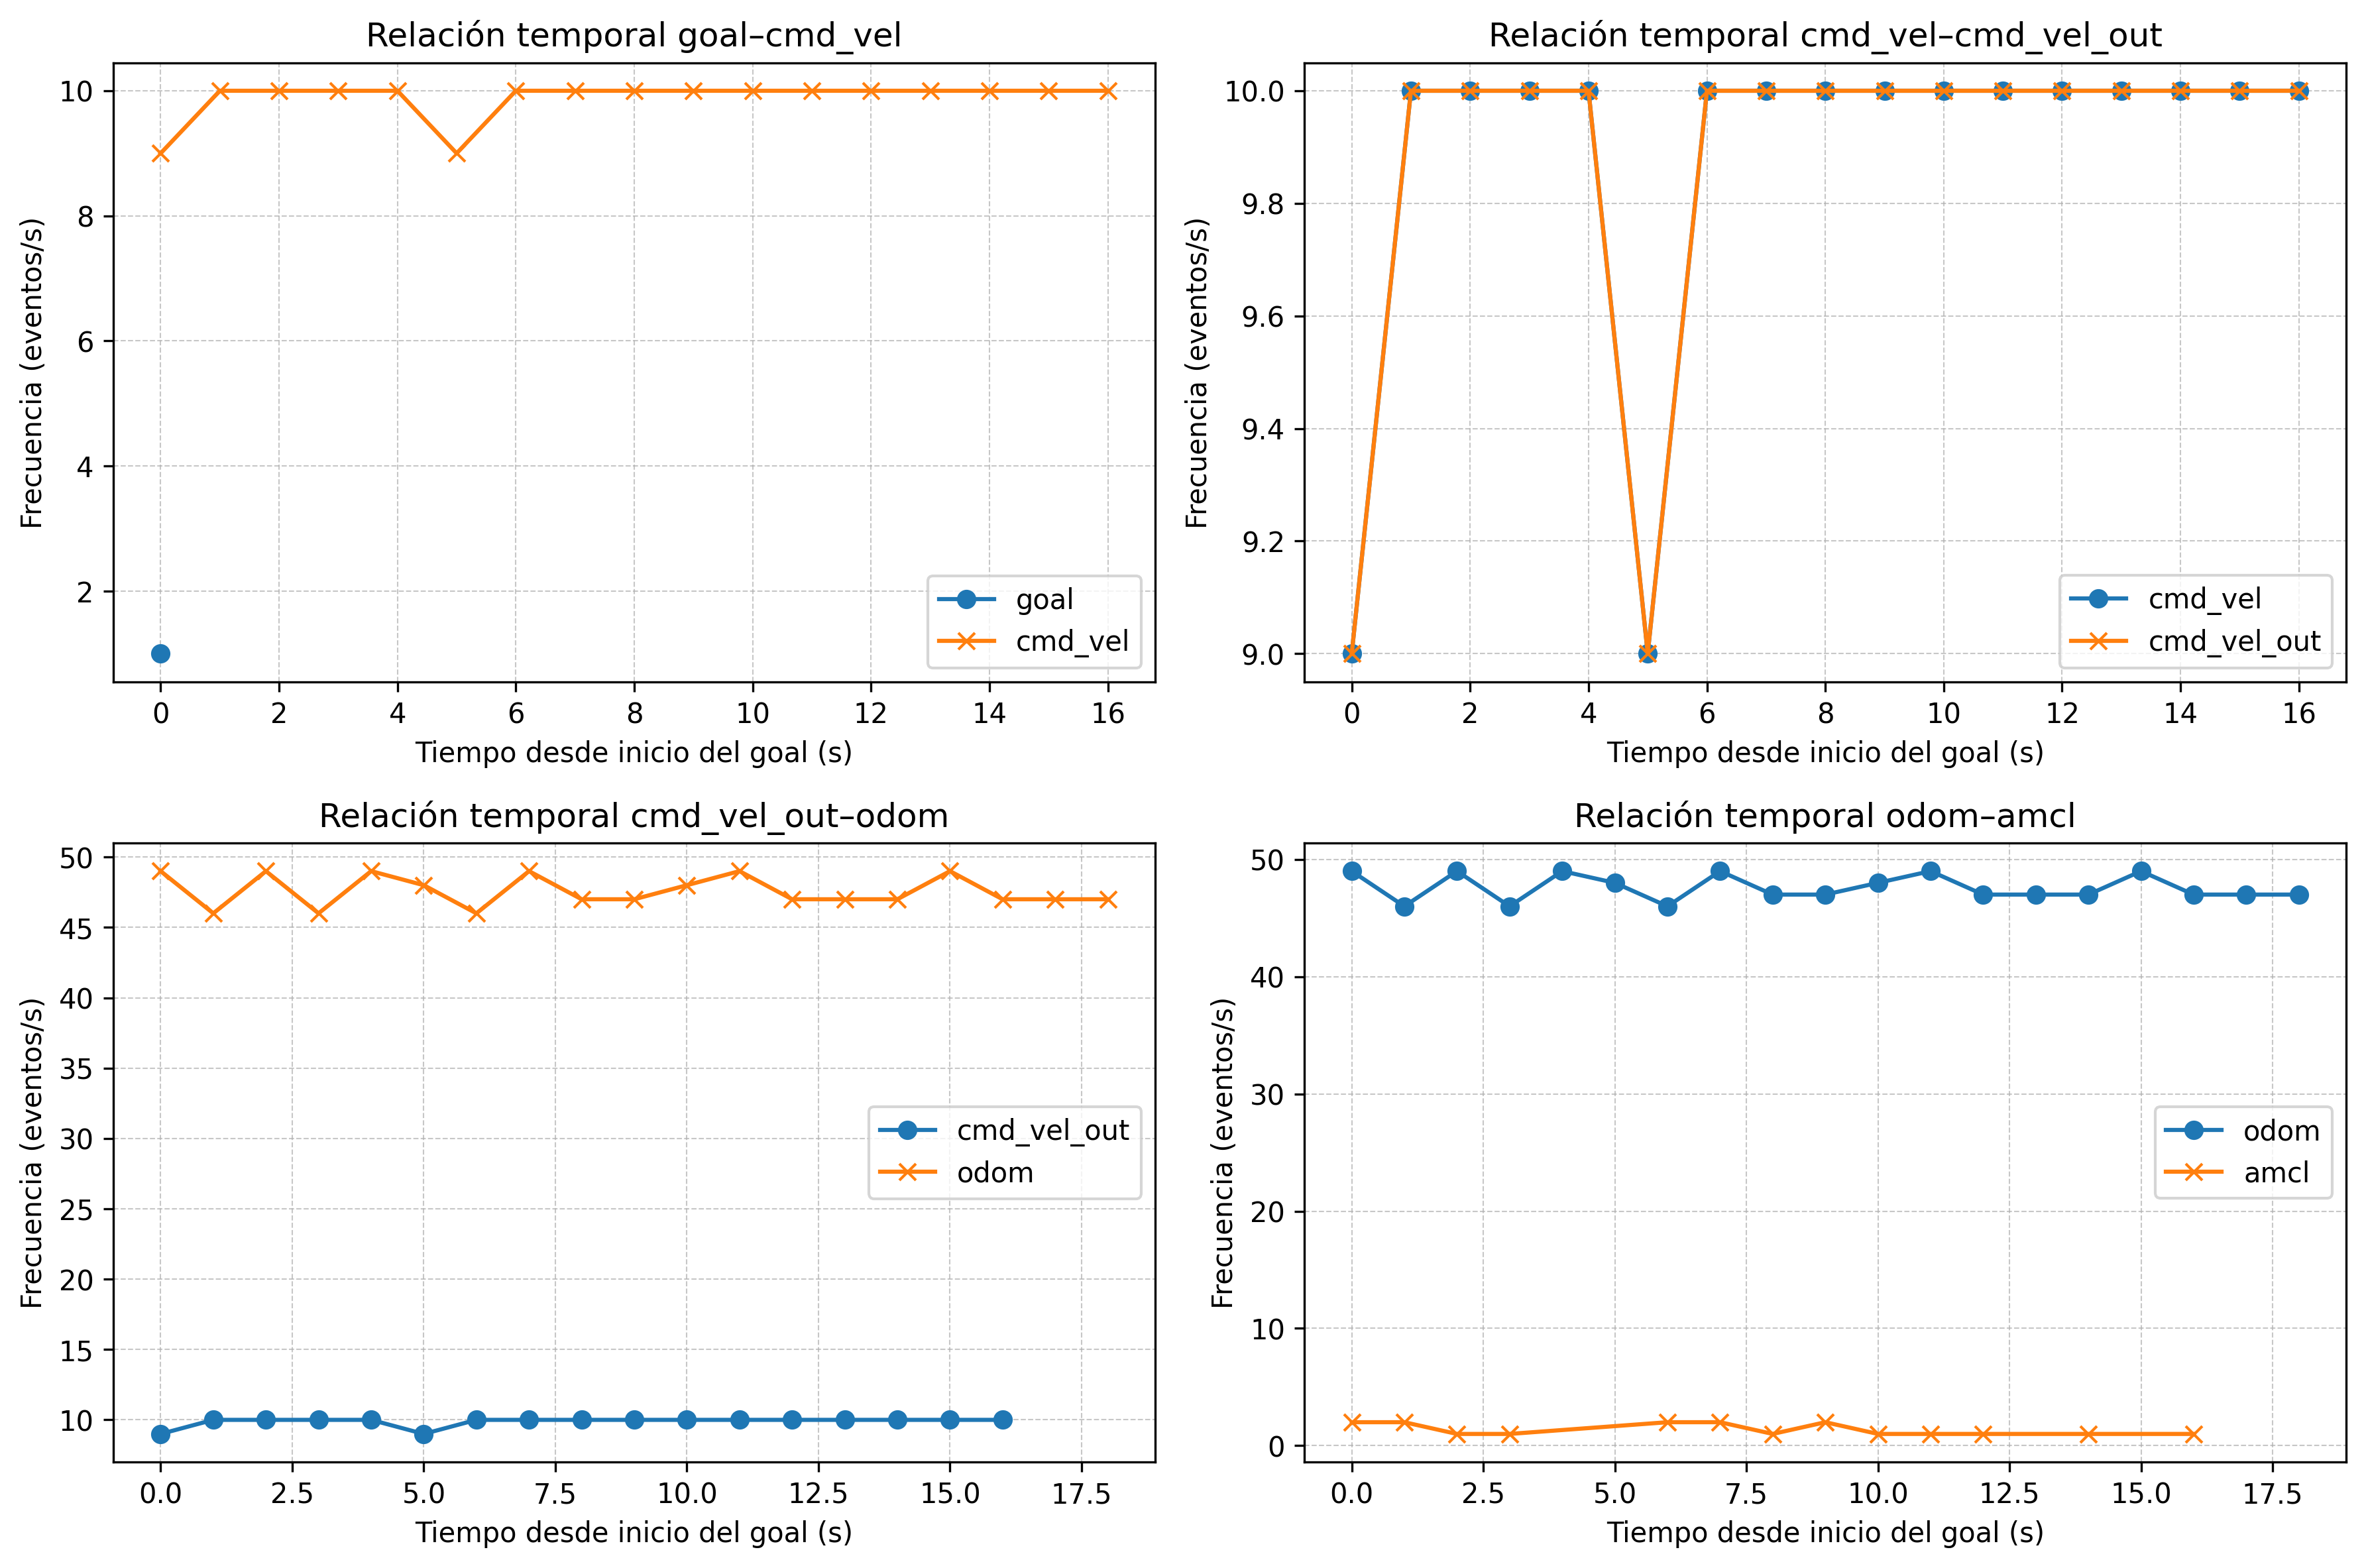
\includegraphics[width=0.9\linewidth]{figures/asynchronous_event_frequencies.png}
    \caption{Frecuencia de publicación de los distintos subsistemas a lo largo del tiempo para un objetivo representativo.}
    \label{fig:asynchronous_event_frequencies}
\end{figure}

No obstante, esta representación constituye una simplificación 
del comportamiento real del sistema. En la práctica, los distintos 
subsistemas operan de forma parcialmente desacoplada, con dependencias 
que se aproximan mejor a una estructura de grafo acíclico dirigido (DAG), 
donde múltiples flujos de información evolucionan de manera asíncrona. 
La interpretación como un modelo lineal event-driven se adopta, por tanto, 
como una aproximación práctica que permite estructurar el análisis, 
asumiendo una relación causal dominante entre eventos.

Esta asincronía se pone de manifiesto en la Figura \ref{fig:asynchronous_event_frequencies}, 
donde se observa un desacoplamiento en las frecuencias de publicación 
de los distintos subsistemas, especialmente en los tramos 
\textit{cmd\_vel\_out--odom} y \textit{odom--amcl}, donde existen relaciones de tipo uno-a-muchos y muchos-a-uno. 
Este comportamiento evidencia la naturaleza asíncrona del sistema. Como consecuencia, la selección de eventos 
basada en el criterio de primer evento posterior puede no capturar 
adecuadamente la correspondencia temporal entre señales.

Para mitigar este efecto, se aplica un tratamiento selectivo de las series temporales mediante 
\textit{Dynamic Time Warping} (DTW), un algoritmo que mide la similitud entre secuencias permitiendo 
deformaciones no lineales en el eje temporal. Este enfoque resulta especialmente adecuado cuando 
existen discrepancias en la frecuencia de eventos, ya que proporciona una alineación 
temporal más consistente entre subsistemas.